\documentclass[../main]{subfiles}
\begin{document}

\chapter{滤波法及数字锁相环法位同步提取}%
\label{cha:pll}

% \section{实验目的}%
% \label{sec:\arabic{chapter}aim}
%
% \begin{itemize}
%   \item 掌握滤波法提取位同步信号的原理及其对信息码的要求。
%   \item 掌握用数字锁相环提取位同步信号的原理。
%   \item 掌握位同步器的同步建立时间、同步保持时间、位同步信号、同步抖动等概念。
% \end{itemize}
%
% \section{实验器材}%
% \label{sec:\arabic{chapter}equipment}
%
% \begin{table}[htbp]
%   \centering
%   \caption{实验器材}%
%   \label{tab:\arabic{chapter}equipment}
%   \csvautobooktabular[respect percent]{tab/\arabic{chapter}equipment.csv}
% \end{table}
%
\section{实验原理}%
\label{sec:\arabic{chapter}principle}

\begin{figure}[htbp]
  \centering
  \begin{subfigure}[htbp]{\linewidth}
    \centering
    \includegraphics[
      width = \linewidth,
    ]{\arabic{chapter}dia/filter}
    \caption{滤波法}%
    \label{fig:tdfm}
  \end{subfigure}

  \begin{subfigure}[htbp]{\linewidth}
    \centering
    \includegraphics[
      width = \linewidth,
    ]{\arabic{chapter}dia/dpll}
    \caption{数字锁相环}%
    \label{fig:itdfm}
  \end{subfigure}
  \caption{实验原理框图}%
  \label{fig:\arabic{chapter}dia}
\end{figure}

将单刀双掷开关 S2 上拨,选择滤波法位同步提取电路,输入 HDB3 单极性码信号经一
个 256K 窄带滤波器,滤出同步信号分量,通过门限判决后提取位同步信号。但由于有
其他频率成分的干扰,导致时钟有些部分的占空比不为 50\%,因此需要通过模拟锁相环
进行平滑处理;

数字的 256K 时钟经过 4 分频之后,已经得到一定的平滑效果,送入 CD4046 鉴相输入
A 脚的是 64KHz 的时钟信号,当 CD4046 处于同步状态时,鉴相器 A 脚的时钟频率及
相位应该与鉴相器 B 脚的相同。由于鉴相器 B 脚的时钟是 VCO 经 8 分频得到的。因
此,VCO 输出的频率为 512K。

锁相法位同步提取是在接收端利用锁相环电路比较接收码元和本地产生的位同步信号的
相位,并调整位同步信号的相位,最终获得准确的位同步信号。4 位拨码开关 S3 设置
BCD 码控制分频比,从而控制提取的位同步时钟频率,例如设置分频频率“0000”输出
4096KHz 频率,“0011”输出 512KHz 频率,“0100”输出 256KHz 频率,“0111”输出
32KHz 频率。

数字锁相环(DPLL)是一种相位反馈控制系统。它根据输入信号与本地估算时钟之间的
相位误差对本地估算时钟的相位进行连续不断的反馈调节,从而达到使本地估算时钟相
位跟踪输入信号相位的目的。DPLL 通常有三个组成模块: 数字鉴相器(DPD)、数字环
路滤波器(DLF)、 数控振荡器(DCO)。根据各个模块组态的不同, DPLL 可以被划分
出许多不同的类型。根据设计的要求,本实验系统采用超前滞后型数字锁相环(LL-DPLL
)作为解决方案。在 LL-DPLL 中,DLF 用双向计数逻辑和比较逻辑实现,DCO 采用“加”
、“扣”脉冲式数控振荡器。这样设计出来的 DPLL 具有结构简洁明快,参数调节方便,
工作稳定可靠的优点。DPLL 实现框图如图~\ref{fig:dpll}。

\begin{figure}[htbp]
  \centering
  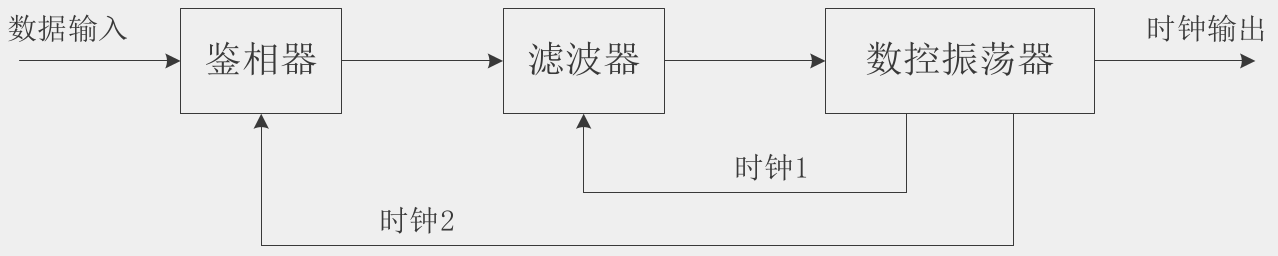
\includegraphics[
    width = 0.8\linewidth,
  ]{dpll}
  \caption{数字锁相环}%
  \label{fig:dpll}
\end{figure}

% 下面就对数字锁相环的各个组成模块的详细功能、内部结构以及对外接口信号进行说明
% :

% \subsection{前-滞后型数字鉴相器}%
% \label{sub:phase_detect}
%
% 与一般 DPLL 的 DPD 的设计不同,位同步 DPLL 的 DPD 需要排除位流数据输入连续几
% 位码值保持不变的不利影响。LL-DPD 为二元鉴相器,在有效的相位比较结果中仅给出相
% 位超前或相位滞后两种相位误差极性,而相位误差的绝对大小固定不变。 LL-DPD 通常
% 有两种实现方式: 微分型 LL-DPD 和积分型 LL-DPD。积分型 LL-DPD 具有优良的抗干
% 扰性能,而它的结构和硬件实现都比较复杂。微分型 LL-DPD 虽然抗干扰能力不如积分
% 型 LL-DPD,但是结构简单,硬件实现比较容易。本实验采用微分型LL-DPD, 将环路抗
% 噪声干扰的任务交给DLF模块负责。
%
% \begin{figure}[htbp]
%   \centering
%   \begin{subfigure}[htbp]{0.45\linewidth}
%     \centering
%     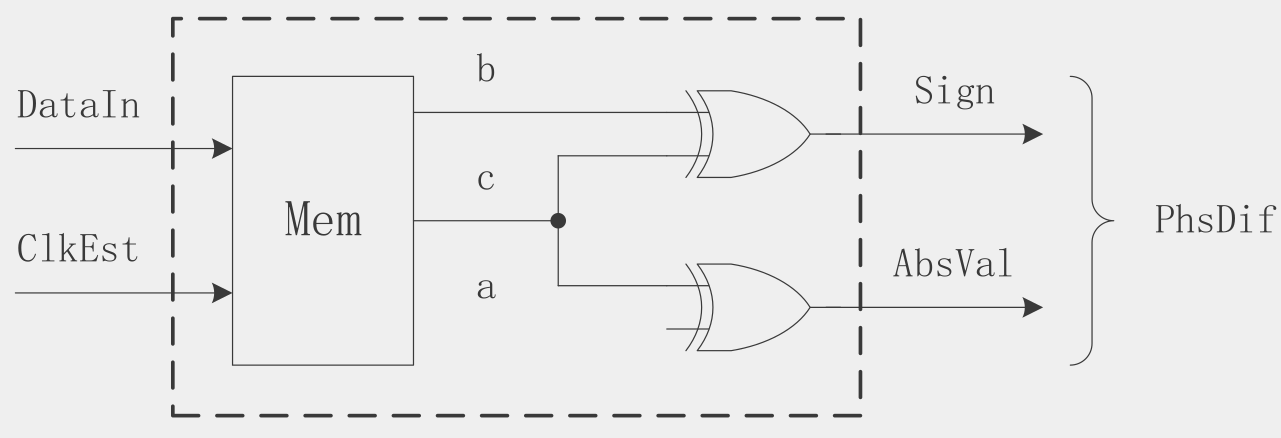
\includegraphics[
%       width = \linewidth,
%     ]{dpd/construction}
%     \caption{内部结构}%
%     \label{fig:dpd/construction}
%   \end{subfigure}
%   \quad
%   \begin{subfigure}[htbp]{0.45\linewidth}
%     \centering
%     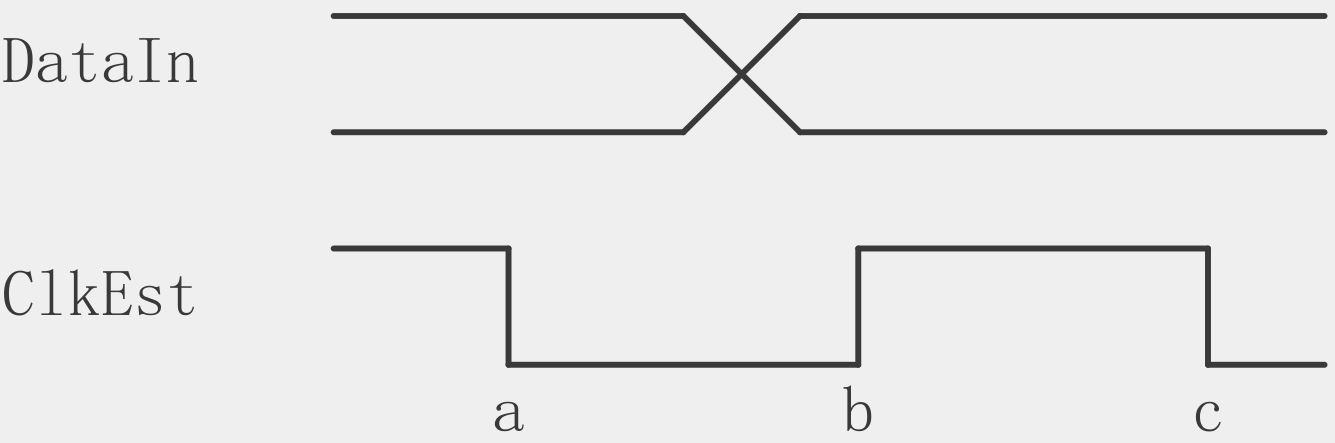
\includegraphics[
%       width = \linewidth,
%     ]{dpd/signal}
%     \caption{信号}%
%     \label{fig:dpd/signal}
%   \end{subfigure}
%   \caption{数字锁相环}%
%   \label{fig:dpd}
% \end{figure}
%
% 如图~\subref{fig:dpd/signal}所示,LL-DPD 在 ClkEst 跳变沿(含上升沿和下降沿
% )处采样 DataIn 上的码值,寄存在 Mem 中。在 ClkEst 下降沿处再将它们对应送到两
% 路异或逻辑中,判断出相位误差信息并输出。 Sign 给出相位误差极性,即 ClkEst 相
% 对于 DataIn 是相位超前(Sign=1)还是滞后(Sign=0)。 AbsVal 给出相位误差绝对
% 值:若前一位数据有跳变,则判断有效,以 AbsVal 输出 1 表示;否则,输出0表示判
% 断无效。图~\ref{fig:dpd}显示了LL-DPD模块的仿真波形图。
%
% \begin{figure}[htbp]
%   \centering
%   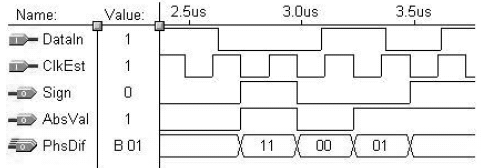
\includegraphics[
%     width = 0.8\linewidth,
%   ]{lldpd}
%   \caption{LL-DPD}%
%   \label{fig:lldpd}
% \end{figure}
%
% \subsection{数字环路滤波器(DLF)}%
% \label{sub:dlf}
%
% DLF 用于滤除因随机噪声引起的相位抖动,并生成控制 DCO 动作的控制指令。本实验实
% 现的 DLF 内部结构及其对外接口信号如图~\ref{fig:dlf}所示。
%
% \begin{figure}[htbp]
%   \centering
%   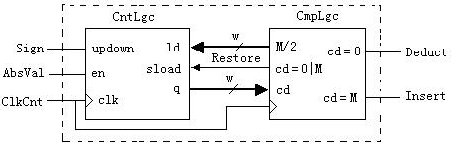
\includegraphics[
%     width = 0.8\linewidth,
%   ]{dlf}
%   \caption{DLF}%
%   \label{fig:dlf}
% \end{figure}
%
% 滤波功能用加减计数逻辑 CntLgc 实现,控制指令由比较逻辑 CmpLgc 生成。在初始时
% 刻, CntLgc 被置初值 M/2。前级 LL-DPD 模块送来的相位误差 PhsDif 在 CntLgc 中
% 作代数累加。在计数值达到边界值 0 或 M 后,比较逻辑 CmpLgc 将计数逻辑 CntLgc
% 同步置回 M/2,同时相应地在 Deduct 或 Insert 引脚上输出一高脉冲作为控制指令。
% 随机噪声引起的 LL-DPD 相位误差输出由于长时间保持同一极性的概率极小,在 CntLgc
% 中会被相互抵消,而不会传到后级模块中去,达到了去噪滤波的目的。计数器逻辑
% CntLgc 的模值 M 对 DPLL 的性能指标有着显著地影响。加大模值 M,有利于提高 DPLL
% 的抗噪能力,但是会导致较大的捕捉时间和较窄的捕捉带宽。减小模值 M 可以缩短捕捉
% 时间,扩展捕捉带宽,但是降低了 DPLL 的抗噪能力。根据理论分析和调试实践,确定
% M 为 1024,图中计数器数据线宽度 w 可以根据 M 确定为 10。
%
% \subsection{数控振荡器}%
% \label{sub:dco}
%
% DCO 的主要功能是根据前级 DLF 模块输出的控制信号 Deduct 和 Insert 生成本地估算
% 时钟 ClkEst,这一时钟信号即为 DPLL 恢复出来的位时钟。同时,DCO 还产生协调
% DPLL 内各模块工作的时钟,使它们能够协同动作。要完成上述功能,DCO 应有三个基本
% 的组成部分:高速振荡器(HsOsc)、相位调节器(PhsAdj)、分频器(FnqDvd),如
% 图~\ref{fig:dco}所示。
%
% \begin{figure}[htbp]
%   \centering
%   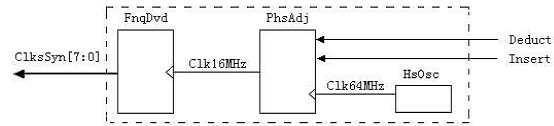
\includegraphics[
%     width = 0.8\linewidth,
%   ]{dco}
%   \caption{DCO}%
%   \label{fig:dco}
% \end{figure}
%
% 高速振荡器(HsOsc)提供高速稳定的时钟信号 Clk,该时钟信号有固定的时钟周期,周
% 期大小即为 DPLL 在锁定状态下相位跟踪的精度,同时,它还影响 DPLL 的捕捉时间和
% 捕捉带宽。考虑到 DPLL 工作背景的要求,以及尽量提高相位跟踪的精度以降低数据接
% 收的误码率,取 HsOsc 输出信号 Clk 频率为所需提取位时钟信号的 16 倍。若取
% HsOsc 输出信号 Clk64MHz 的周期为 15.625ns,即高速振荡器 HsOsc 的振荡频率为
% 64MHz。
%
% PhsAdj 在控制信号 Deduct 和 Insert 上均无高脉冲出现时,仅对 Osc 输出的时钟信
% 号作 4 分频处理,从而产生的 Clk16MHz 时钟信号将是严格 16MHz 的。当信号 Deduct
% 上有高脉冲时,在脉冲上升沿后,PhsAdj 会在时钟信号 Clk16MHz 的某一周期中扣除一
% 个 Clk64Mhz 时钟周期,从而导致 Clk16MHz 时钟信号相位前移。当在信号 Insert 上
% 有高脉冲时,相对应的处理会导致 Clk16MHz 时钟信号相位后移。图~\ref{fig:phsadj}
% 为相位调节器单元经功能编译仿真后的波形图。
%
% \begin{figure}[htbp]
%   \centering
%   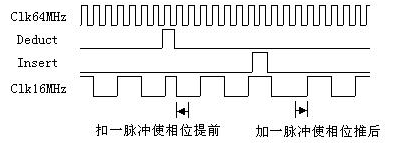
\includegraphics[
%     width = 0.8\linewidth,
%   ]{phsadj}
%   \caption{phsadj}%
%   \label{fig:phsadj}
% \end{figure}
%
% 引入分频器 FnqDvd 的目的主要是为 DPLL 中 DLF 模块提供时钟控制,协调 DLF 与其
% 它模块的动作。分频器 FnqDvd 用计数器实现,可以提供多路与输入位流数据有良好相
% 位同步关系的时钟信号。在系统中,分频器 FnqDvd 提供 8 路输出
% ClksSyn$[7..0]$。其中,ClksSyn1 即为本地估算时钟 ClkEst,也即恢复出的
% 位时钟;ClksSyn0 即为 DLF 模块的计数时钟 ClkCnt,其速率是 ClkEst 的两倍,可以
% 加速计数,缩短 DPLL 的捕捉时间,并可扩展其捕捉带宽。
%
\section{实验步骤}%
\label{sec:\arabic{chapter}procedure}

\subsection{滤波法位同步电路带通滤波器幅频特性测量}%
\label{sub:bpf}

% 该项目是通过改变输入信号的频率,观测信号经滤波后对应输出幅度,从而了解并绘制
% 滤波器的幅频特性。

% \begin{table}[htbp]
%   \centering
%   \caption{连线}%
%   \label{tab:\arabic{chapter}\arabic{subsection}}
%   \csvautobooktabular[respect percent]{tab/\arabic{chapter}\arabic{subsection}.csv}
% \end{table}

% \begin{enumerate}
%   \item 关电,按表~\ref{tab:\arabic{chapter}\arabic{subsection}}所示进行连线。
%   \item 开电,设置主控,选择【信号源】→【输出波形】。设置输出波形为正弦波,调
%     节相应旋钮,使其输出频率为 200KHz,峰峰值 3V。
%   \item 此时系统初始状态为:输入信号为频率 200KHz、幅度 3V 的正弦波。
%   \item 实验操作及波形观测。

分别观测 13 号模块的“滤波法位同步输入”和“BPF-Out”,改变信号源的频率,测量
“BPF-Out”的幅度填入表,并绘制幅频特性曲线图~\ref{fig:bp}。
% \end{enumerate}

% \begin{table}[htbp]
%   \centering
%   \caption{幅频特性}%
%   \label{tab:bp}
%   \csvautobooktabular[respect percent]{tab/bp.csv}
% \end{table}

\begin{figure}[htbp]
  \centering
  \includegraphics[
    width = 0.8\linewidth,
  ]{bp}
  \caption{幅频特性曲线,带宽大约 30dB}%
  \label{fig:bp}
\end{figure}

\subsection{滤波法位同步恢复观测}%
\label{sub:bit}

% 该项目是通过比较和观测滤波法位同步电路中各点幅度及相位,探讨滤波法位同步的提
% 取原理以及影响因素。

% \begin{table}[htbp]
%   \centering
%   \caption{连线}%
%   \label{tab:\arabic{chapter}\arabic{subsection}}
%   \csvautobooktabular[respect percent]{tab/\arabic{chapter}\arabic{subsection}.csv}
% \end{table}

% \begin{enumerate}
%   \item 关电,按表格所示进行连线。
%   \item 开电,设置主控菜单,选择【信号源】→【通信原理】→【滤波法及数字锁相环位同步法提取】。将 13 号模块 S2 拨上。将 S4 拨为 1000。
%   \item 此时系统初始状态为:输入 PN 为 256K。
%   \item 实验操作及波形观测。
\begin{enumerate}
  \item 观测“门限判决输出”,记录波形图~\ref{fig:filter/judge}。

    \begin{Exercise}[title = 思考, label = ex:\arabic{chapter}\arabic{Exercise}]
      分析在什么情况下门限判决输出的时钟会不均匀,为什么?
    \end{Exercise}

    \begin{Answer}
      当信号含有丰富的谐波分量时,信号复杂,频率分量较多时。另外带通滤波器带
      宽较大时会有极大概率判决出错。时钟信号会不均匀。例如
      图~\ref{fig:filter/judge}左边比右边略微宽一点。
    \end{Answer}

  \item 观测“鉴相输入 1”,记录波形图~\ref{fig:filter/phase}。
  \item 对比“门限判决输出”和“鉴相输入 1”的波形图~\ref{fig:filter/compare}。

    \begin{Exercise}[title = 思考, label = ex:\arabic{chapter}\arabic{Exercise}]
      分析时钟不均匀的情况是否有所改善。
    \end{Exercise}

    \begin{Answer}
      有所改善,占空比接近50\%。由图~\ref{fig:\arabic{chapter}dia}可见,信号
      存在四分频的步骤。四个周期的累加使得时钟有所改善。
    \end{Answer}

  \item 对比观测“鉴相输入 1”和“鉴相输入 2”,记录波形
    图~\ref{fig:filter/compare_phase}。比较两路波形的幅度和相位。
  \item 对比观测“滤波法位同步输入”和“BS1”图~\ref{fig:filter/compare_bs},观测
    恢复的位同步信号。
\end{enumerate}
% \end{enumerate}

\begin{figure}[htbp]
  \centering
  \begin{subfigure}[htbp]{0.45\linewidth}
    \centering
    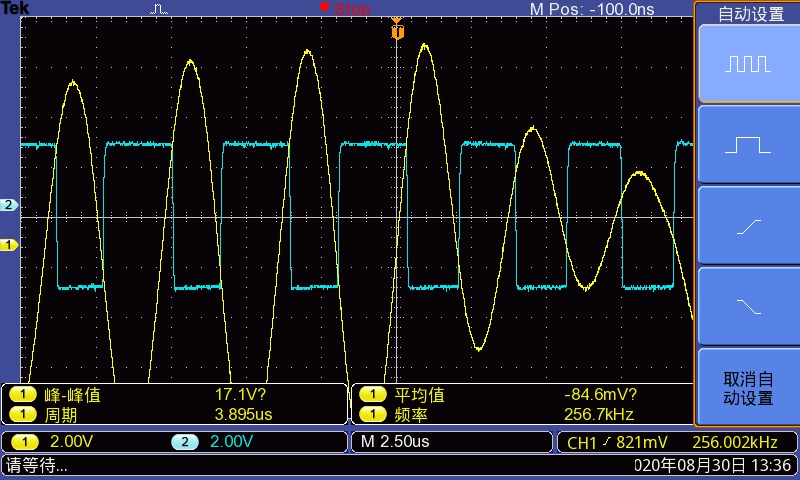
\includegraphics[
      width = \linewidth,
    ]{filter/judge}
    \caption{判决输出}%
    \label{fig:filter/judge}
  \end{subfigure}
  \quad
  \begin{subfigure}[htbp]{0.45\linewidth}
    \centering
    \includegraphics[
      width = \linewidth,
    ]{filter/phase}
    \caption{鉴相输入}%
    \label{fig:filter/phase}
  \end{subfigure}

  \begin{subfigure}[htbp]{0.45\linewidth}
    \centering
    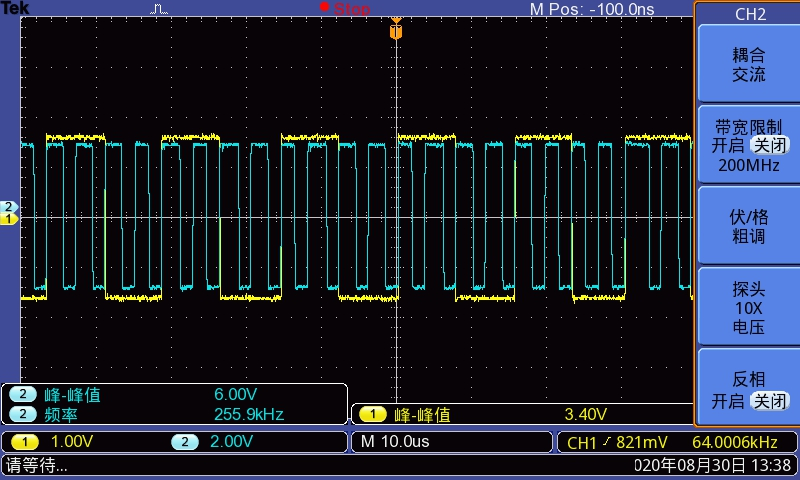
\includegraphics[
      width = \linewidth,
    ]{filter/compare}
    \caption{对比判决输出和鉴相输入}%
    \label{fig:filter/compare}
  \end{subfigure}
  \quad
  \begin{subfigure}[htbp]{0.45\linewidth}
    \centering
    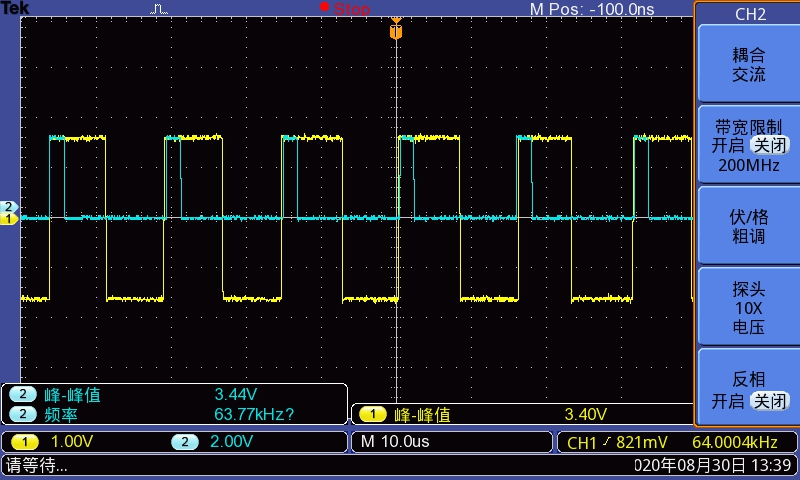
\includegraphics[
      width = \linewidth,
    ]{filter/compare_phase}
    \caption{对比鉴相输入}%
    \label{fig:filter/compare_phase}
  \end{subfigure}

  \begin{subfigure}[htbp]{0.45\linewidth}
    \centering
    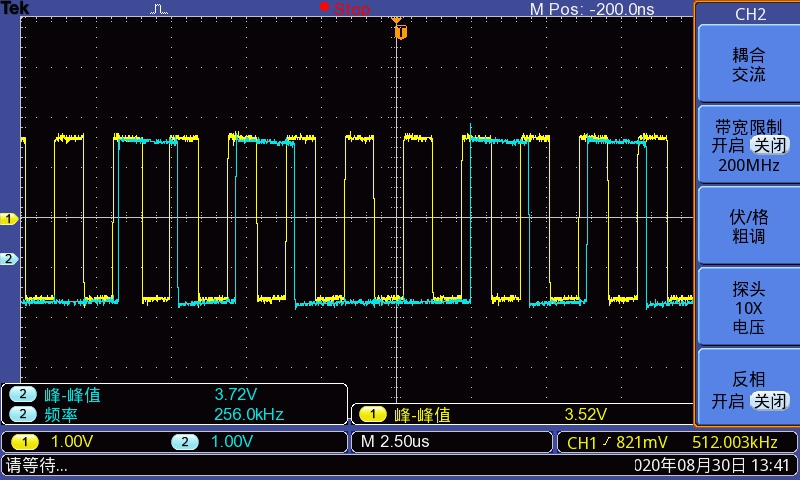
\includegraphics[
      width = \linewidth,
    ]{filter/compare_bs}
    \caption{对比输入和 BS1}%
    \label{fig:filter/compare_bs}
  \end{subfigure}
  \caption{滤波法位同步恢复观测}%
  \label{fig:filter}
\end{figure}

\subsection{数字锁相环法位同步观测}%
\label{sub:dpll}

% 该项目是通过比较和观测数字锁相环位同步电路中各点相位超前、延时以及抖动情况,
% 探讨数字锁相环法位同步的提取原理。

% \begin{table}[htbp]
%   \centering
%   \caption{连线}%
%   \label{tab:\arabic{chapter}\arabic{subsection}}
%   \csvautobooktabular[respect percent]{tab/\arabic{chapter}\arabic{subsection}.csv}
% \end{table}

% \begin{enumerate}
%   \item 关电,按表~\ref{tab:\arabic{chapter}\arabic{subsection}}所示进行连线。
%   \item 开电,设置主控菜单,选择【信号源】→【通信原理】→【滤波法及数字锁相环位同步法提取】。将 13 号模块的 S3 拨为 0100。
%   \item 此时系统 初始状态为: PN 码速率 256K。
%   \item 实验操作及波形观测。
\begin{enumerate}
  \item 观测 13 模块的“数字锁相环输入”和“鉴相输出”。观测相位超前滞后的情况
    图~\ref{fig:pll/phase}。
  \item 观测 13 模块的“插入指示”和“扣除指示”图~\ref{fig:pll/insert_subtract}。

    \begin{Exercise}[title = 思考, label = ex:\arabic{chapter}\arabic{Exercise}]
      分析波形有何特点,为什么出现这种情况。
    \end{Exercise}

    \begin{Answer}
      插入指示和扣除指示波形相同,都是由脉宽小的周期性脉冲信号组成。因为插入
      指示和扣除指示是数字信号振荡器的控制信号,为了方便识别(与噪声信号分开
      ),所以设计成了持续时间短,幅度高的周期脉冲信号。
    \end{Answer}

  \item 观测 13 号模块的“BS2”图~\ref{fig:pll/bs2}。
\end{enumerate}
% \end{enumerate}

\begin{figure}[htbp]
  \centering
  \begin{subfigure}[htbp]{0.45\linewidth}
    \centering
    \includegraphics[
      width = \linewidth,
    ]{pll/phase}
    \caption{相位超前滞后}%
    \label{fig:pll/phase}
  \end{subfigure}
  \quad
  \begin{subfigure}[htbp]{0.45\linewidth}
    \centering
    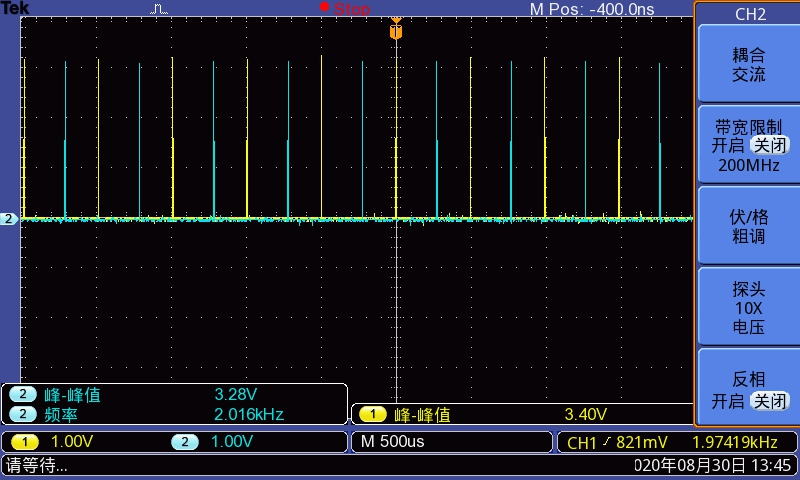
\includegraphics[
      width = \linewidth,
    ]{pll/insert_subtract}
    \caption{插入指示和扣除指示}%
    \label{fig:pll/insert_subtract}
  \end{subfigure}

  \begin{subfigure}[htbp]{0.45\linewidth}
    \centering
    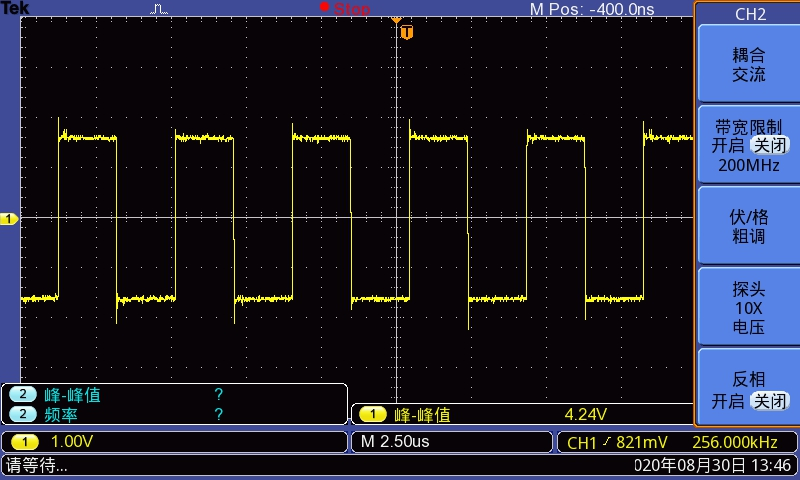
\includegraphics[
      width = \linewidth,
    ]{pll/bs2}
    \caption{BS2}%
    \label{fig:pll/bs2}
  \end{subfigure}
  \caption{锁相环法}%
  \label{fig:pll}
\end{figure}

\begin{Exercise}[title = 思考, label = ex:\arabic{chapter}\arabic{Exercise}]
  BS2 恢复的时钟是否有抖动的情况,为什么?试分析 BS2 抖动的区间有多大?如何减
  小这个抖动的区间?
\end{Exercise}

\begin{Answer}
  有抖动现象。因为可变分频器是非相参的,所以无法确定下一个时钟沿的到达时间。
  抖动区间是可变分频器的周期。可以通过增大分频系数减小这个区间。
\end{Answer}

\section{实验报告}%
\label{sec:\arabic{chapter}report}

\begin{Exercise}
  对实验思考题加以分析,按照要求做出回答,并尝试画出本实验的电路原理图。
\end{Exercise}

\begin{Answer}
  思考题见问题~\ref{ex:\arabic{chapter}1}、\ref{ex:\arabic{chapter}2}、\ref{ex:\arabic{chapter}3}、\ref{ex:\arabic{chapter}4},回答见回答~\ref{ex:\arabic{chapter}1}、\ref{ex:\arabic{chapter}2}、\ref{ex:\arabic{chapter}3}、\ref{ex:\arabic{chapter}4}。
  电路原理图见图~\ref{fig:\arabic{chapter}dia}。
\end{Answer}

\begin{Exercise}
  结合实验波形分析数字锁相环原理。
\end{Exercise}

\begin{Answer}
  原理见章节~\ref{sec:\arabic{chapter}principle}。

  分析:数字锁相环由鉴相器、环路滤波器、数字控制振荡器。鉴相器在每一个周期内
  将输入信号与本地时钟进行相位比较,相位误差经过环路滤波后消除噪声控制数字控
  制振荡器产生振荡(插入或扣除脉冲),从而产生本地时钟信号。本质上是一个闭环
  负反馈。
\end{Answer}

\end{document}
